%%%%%%%%%%%%%%%%%%%%%%%%%%%%%%%%%
%%%%% SECTION %%%%%%%%%%%%%%%%%%%
%%%%%%%%%%%%%%%%%%%%%%%%%%%%%%%%%

\section{Command and Control}

The definition of C2 originally referred to the classical military strategies applied in the XIX and XX centuries, with a central commander and an inflexible hierarchical chain of command~\cite{Alberts2006}. However, this concept is totally incompatible with the modern warfare and environment, where information sharing causes impacts over the results.

The \gls{DoD}~\cite{dod01} defines C2 as the exercise of authority and direction by a properly designated commander over assigned and attached forces in the accomplishment of the mission. However, this definition does not permit to identify the existence of C2 in the organization and to perform its assessment. Furthermore, it is limited in terms of research aspects and does not involves many other C2 applications in all possible contexts. It is more compatible when we have a static scenario where changes do not occur. In this case, the entities involved have predictable behavior and it is not required to have a mechanism to do a constant monitoring. 

NATO extended this definition to the functions of commanders, staffs, and other Command and Control bodies in maintaining the combat readiness of their forces, preparing operations, and directing troops in the performance of their tasks~\cite{FRANCE2014}. With this, C2 becomes a concept that naturally involves a dynamic context because it empowers the system with the capacity to deal with changes in circumstances~\cite{Power01}.

According to \textit{Stanton et al.}~\cite{Stanton2007} and \textit{Mason et al.}~\cite{Mason2001}, C2 relies on information and awareness sharing rather than simply data broadcast. Information needs to respect the rules and logical conditions to reach the right target and to cause the right effect. This information sharing occurs on a network structure that satisfies the context requirements, including mission details and context restrictions. 

Empower the individuals on the edge of the organization, spreading the information in the right way and compatible quantity, is the new challenge to support a wider C2 definition. \textit{Alberts and Hayes} in \cite{Power01} presented the term \textit{Power to the Edge} aiming to expose the idea of take the information to all elements in the organization. It is directly related to the information and awareness spread level.

The same work~\cite{Power01} presented the three key dimensions of C2: Allocation of Decision Rights, Patterns of Interaction and Distribution of Information. These dimensions, not completely independent, compose the C2 Approach Space described by \textit{Alberts et al.} in \cite{Alberts2006} show in Figure \ref{c2s}.

\figura[!h]{C2_Space}{C2 Approach Space (from \cite{FRANCE2014})}{c2s}{width=0.6\textwidth}%

\textbf{a) Allocation of Decison Rights (ADR)}

Decision rights are the capability of some individuals to make choices related to a specific topic. The allocation of this capability aims the unity of purpose. With the ADR more distributed, the leadership changes according to the information shared.

The ADR axis represents, in an endpoint, the total centralization of decision rights, and in the other end of the spectrum, the total capability to take decisions for all members. In this case, no leadership is identified.

\textbf{b) Patterns of Interaction (PoI)}

Basically, PoI defines the network topology used by the entities. According to \textit{Alberts and Hayes} in~\cite{Alberts2006}, it is possible to identify four different types of networks, not related to hierarchy, that makes an approach of C2 in Information age militaries.

\begin{itemize}
    \item Fully connected: every entity is connected to every other, or there is an interaction among all of them;
    \item Random networks: each entity has the same probability of interacting with any other;
    \item Scale-free networks: a few entities have a very large number of connections or interactions with other entities;
    \item Small world networks: very high cluster coefficient, with a number of connections around $log(N)$, where $N$ is the total of nodes \cite{small01}.
\end{itemize}
 
The richest network structure is that mixed with different types in each level\cite{Alberts2006}. It should be the one with a scale-free in high level, the intermediate level composed by small world networks and at local level, the using of fully connected network structure.

\textit{Zughe and Sun} \cite{small02} proposed a solution to represent a Small-World network using a virtual ring topology. In that work, it is presented some aspects that permits a simpler approach to represent this kind off communication strucutre.

\textbf{c) Distribution of Information (DoI)}

How the information is shared, following the Information Exchange Requirements (IRE) and get the shared awareness. Based on this, it is presented a conceptual model to C2 Agility, that is the capability of C2 to successfully effect, cope with or exploit changes in circumstances.\cite{ABAR201713} 



%%%%%%%%%%%%%%%%%%%%%%%%%%%%%%%%%
%%%%%%%%%%%%%%%%%%%%%%%%%%%%%%%%%

\subsection {Network Enabled Capabilities}

The Network Enabled Capabilities - NCW (England) or Network Centric Warfare (USA) - NEC was created to increase the action power through a shared awareness that can be synchronized using a specific network structure and organization to create entities interaction \cite{Alberts2000}. 

Based on NEC paradigm, it was identified five archetypes to C2 Approach. These archetypes are listed in Table \ref{table:nec} and are defined as \gls{C2 Strategy} with their characteristics. Each \gls{C2 Strategy} adopted is related to a certain maturity level and occupies a specific position in C2 Approach Space.

\begin{table}[ht]
	\small
	\fontsize{6}{6}\selectfont
	\centering
	\caption{Network types associated to C2 Approaches}
	\label{table:nec}
	
	\begin{tabular}{p{0.1\linewidth}p{0.5\linewidth}p{0.2\linewidth}p{0.1\linewidth}}
	\hline
		\textbf{NEC Approach (C2 archetypes)}
		& \textbf{Archetype Characteristics}
		& \textbf{Network Type}
		& \textbf{Topology} \\ [1ex]
	\hline	
	Edge C2 & All elements are connected to everyone; There are $\frac{n(n-1)}{2}$ connections & Fully connected & Fully Connected \\[5ex]
	Collaborative C2 & Shared resources; entities interdependence; suitable to holistic problems that can not be fully decomposed; peer-to-peer communication & Scale-free Networks (a few nodes have a very large number of connections) & Star + Fully connected \\[5ex]
	Coordinated C2 & Suitable to problems that can be fully decomposed; share necessary information to execute what was defined & Random Networks (same probability to connect) & Star \\[5ex]
	De-Conflicted C2 & The situation can be decomposed with no cross impact; sub-optimized; not suitable to dynamic scenarios & Small World Networks ( $\log{N}$ connections & Ring \\[5ex]
	Conflicted C2 & No communication between entities & Isolated & - \\[1ex]
	\hline
	\end{tabular}
\end{table} 



The term Network Enabled Capability (NEC) looks for achieving the effect with the best usage of information systems. \textit{Alberts et al.} presented~\cite{nato01} the five NATO NEC C2 Maturity levels that represents a number of C2 Approaches to deal with different contexts as listed below.

\begin{itemize}
    \item Edge C2
    \item Collaborative C2
    \item coordinated C2
    \item De-Conflicted C2
    \item Conflicted C2
\end{itemize}

Each of these approaches corresponds to a specific region in the C2 Approach Space as shown in Figure \ref{c2s02}.

\figura[ht]{C2S_02}{NEC Approaches to C2 (from \cite{FRANCE2014})}{c2s02}{width=0.7\textwidth}%

These approaches are selected according to the mission and a set of circumstances. Different context requires specific \gls{C2} approaches. When some of these elements change, it is possible that some C2 approaching is not suitable anymore. The set of possible approaches available to be employed defines the Endeavor Space~\cite{FRANCE2014}.

SAS-060 \cite{nato01}, by \gls{NATO}, recommended following transition rules in case of endeavor complexity  changes showed in Table \ref{table:table02}.

\begin{table}[ht]
	\small
	\fontsize{10}{10}\selectfont
	\centering
	\caption{Endeavour complexity  changes}
	\label{table:table02}
	
	\begin{tabular}{ccccc}
	\hline
		\textbf{Endeavour Complexity}
		& \textbf{Appropriate C2 Approach} \\ [1ex]
	\hline	
	
	Low & De-conflicted \\[1ex]
	Medium & Coordinated \\[1ex]
	Medium-High & Collaborative \\[1ex]
	High - Very High & Edge \\[1ex]
	\hline
	\end{tabular}
\end{table} 

Communications improvements conduct the entities to a C2 Approach closer to the edge. This more connected structure becomes the awareness spread easier, due to the information sharing and collaboration among entities. The network structure and robustness facilitate to share awareness among dispersed entities. 


%%%%%%%%%%%%%%%%%%%%%%%%%%%%%%%%%
%%%%%%%%%%%%%%%%%%%%%%%%%%%%%%%%%

\subsection{Endeavor Space}

The set of all requirements, circumstances and conditions of a mission forms the endeavor space. It is created when all possible changes in circumstances that may cause impacts in an entity, and these possibilities are systematically identified and mapped ~\cite{FRANCE2014}. 

Precisely, the Endeavor Space is identified during planning time to try to preview the changes in circumstances as more precise as possible. It reduces the inherent uncertainties during mission execution~\cite{FRANCE2014}.

Each region of the endeavor space requires an option in C2 Approach Space to deal with the challenges and to perform the mission given. Different circumstances and other context changes implies in different regions in endeavor space.

A computational view of endeavor space is a search space to the C2 functions application. At different moments, these functions have a specific region of endeavor space as domain values, that conduct to the result or objective, e.g., mission accomplishment. The area formed by the sum of all regions where an entity operates defines the entity's agility in a general way \cite{Alberts2011}.

Based on the domain studies, these changes in circumstances that conduct to different endeavor space positions and these changes can be divided in three different areas: self, environment and mission~\cite{Alberts2006}.

%%%%%%%%%%%%%%%%%%%%%%%%%%%%%%%%%
%%%%%%%%%%%%%%%%%%%%%%%%%%%%%%%%%

\subsection {Functions of C2}

A C2 application permits the identification of some related functions that are required in order to apply C2 concepts and principles~\cite{Alberts2006}. These functions are listed bellow and are applicable to many endeavor types (military, civilian and industrial). They are related to C2 and describe the steps to be fellow:
\begin{itemize}
    \item Establishing intent
    \item Determining roles
    \item Establishing rules and constraints
    \item Monitoring and assessing the situation and the progress
\end{itemize}

However, it is necessary to consider the leadership factor. How the commanders or managers are good as leaders guiding the team to the mission or task accomplishment. To this aspect, it is necessary to add the following functions:

\begin{itemize}
    \item Inspiring, engendering trust and motivating
    \item Training and education
    \item provisioning
\end{itemize}

These three last functions are related to human aspects and behaviors. They depend on the actor that are as commander or manager.





%%%%%%%%%%%%%%%%%%%%%%%%%%%%%%%%%
%%%%% SECTION %%%%%%%%%%%%%%%%%%%
%%%%%%%%%%%%%%%%%%%%%%%%%%%%%%%%%

\subsection {\gls{C2 Agility}}

Agility can be defined as a capability to deal with different circumstances, adapting to new requirements, to continue the tasks execution. Figures \ref{graph01} and \ref{graph02} depict situations where the identification of abnormalities was not effective and results were out of acceptance level. \textit{Alberts et al.}~\cite{Alberts2011} defines agility of an entity as the area inside the endeavor space that it is capable to act according to the requirements.

\figura[!h]{graph01}{Lack of agility demanding a long time to react to an abnormality (adapted from \cite{FRANCE2014})}{graph01}{width=.8\textwidth}%
\figura[!h]{graph02}{Agility characterized by a fast response under circumstance changes (adapted from~\cite{FRANCE2014})}{graph02}{width=.8\textwidth}%

To be considered agile, the Entity must to be able to detect an event and to adopt some action to keep results in satisfactory levels. This indicates an Entity's responsiveness compatible with dynamic \gls{context}.

\gls{c2agility} is a function of C2 approach agility and \gls{C2 Maneuver} agility and represents the capability of an entity to adapt itself to deal with different circumstances. This adaptation can be done through a fine tune with no C2 Approach change to improve capabilities, featuring what is shown in Figure \ref{fig100}. In case of adaptation within the same C2 Approach, this adaptation can be expressed as an entity reconfiguration or tasks reallocation.

However, the new circumstance can require a deeper adaptation and in this case, a C2 Approach change will occur to deal with new requirements. Figure \ref{fig101} represents this last agility where it is mandatory to perform a C2 maneuver as fast as possible.

To provide C2 Agility, it is fundamental a fast \textit{sensemaking} \cite{Power01}, i.e., situational awareness, to get a right decision into the scenario to execute the right actions aiming to solve the problems. It is a requirement to any action to be adopted in a real situation. In a automated system, it is obtained by sensors able to get information from the environment and from themselves to adapt the system according to the circumstance changes. 

\figura[!h]{fig100}{C2 Approach Agility satisfying new requirements with no C2 Approach change}{fig100}{width=.6\textwidth}%
\figura[!h]{fig101}{C2 maneuver performing a C2 Approach change due to new circumstances}{fig101}{width=.6\textwidth}%

To guarantee C2 Agility, it is necessary to have situation awareness and self-monitoring. These two elements permit C2 Approach changes within the C2 Approach Space according to the circumstances. NATO NEC Maturity Model divided the C2 approach space in five regions as cubes that corresponds to specific C2 approaches that can be adopted~\cite{FRANCE2014}. 

All entities have a set of possible C2 Approach that can be adopted during context changes to satisfy new requirements. This capacity is expressed as the ability to recognize the context changes and the incompatibility of the C2 Approach currently applied, tto identify an adequate C2 Approach according to the new circumstance, and to change to this new C2 Approach selected within the time slice previously defined. Figure \ref{c2sm} shows the common movement inside the C2 Approach Space changing the C2 Approach adopted to deal with new circumstances.

\figura[ht]{C2_Space_M}{C2 Approach changes within C2 Approach Space (from \cite{FRANCE2014})}{c2sm}{width=0.6\textwidth}%

The C2 agility can be improved if the capacity to switch between different C2 Approaches is increased. The C2 Approach adopted is related to the endeavor space complexity, being more connected, e.g., Edge, when that complexity gets higher.

Equation \ref{c2a1} shows the C2 agility metric representation, proposed by \textit{Alberts}~\cite{Alberts2017}, by the relation between the endeavor space were the entities are able to act, and the total endeavor space area. The endeavor space portions \textit{S1, S2} and \textit{S3} are three regions inside the endeavor space that the entities can act according to some quality parameters, e.g., effectiveness and timeliness. 

\begin{equation}
\label{c2a1}
 C2_{metric} = \frac{S1 + S2 + S3}{endeavor\ space}  
\end{equation}

The maturity levels presented by NATO in SAS-065 report~\cite{nato01}, i.e., the five C2 Approaches previously mentioned, represent the ability of an entity or a group of entities to change the C2 Approach under circumstances changes. However, the first step to perform a maneuver within the C2 Approach Space is to identify what is the current position in this space. C2 Agility will guarantee the right position in the C2 Approach space during the mission execution under context changes. When the circumstances' requirements cause a significant location change within the endeavor space, there is a mapping to a different region and consequently we have a C2 Approach modification. 

In C2, the \gls{agility} is linked with agile forces and operational concepts. The six components of agility, that combines agile individuals, organizations and C2 Systems, are listed bellow~\cite{Power01}:

\begin{itemize}
    \item \textbf{Robustness:}it is the ability to maintain the effectiveness across a range of tasks, conditions and situations;
    \item \textbf{Resilience:} it is the ability to recover or adjust from a damage or perturbation in the environment;
    \item \textbf{Responsiveness:} it is the ability to react to a change in the environment in a suitable interval of time;
    \item \textbf{Flexibility:} it is the ability to employ multiple ways to succeed and the capacity to switch between these ways;
    \item \textbf{Innovation:} it is the ability to do new things or in different ways;
    \item \textbf{Adaptation:} it is the ability to change the organization or the processes.
\end{itemize}

These components are called agility enablers, and the combination of these enablers in different levels provide a given agility capacity\cite{FRANCE2014}.

C2 Agility relates the entities available and the mission challenges with a correct C2 approach for each situation. In dynamic scenarios, this agility is required to keep the mission execution. The changes of C2 approaches defines the maneuver in C2 space. This ability to maneuver in the C2 Approach Space involves the significance recognition of circumstance modifications that affect the effectiveness of an approach, and the necessity to change another one more suitable to the new situation.


%%%%%%%%%%%%%%%%%%%%%%%%%%%%%%%%%
%%%%% SECTION %%%%%%%%%%%%%%%%%%%
%%%%%%%%%%%%%%%%%%%%%%%%%%%%%%%%%

\section {Self-Adaptive Systems}

Laddaga et al. in \cite{SAS01} presented the following definition to self-adaptive system (SAS):

\textit{``Self-adaptive software evaluates its own behavior and changes behavior when the evaluation indicates that it is not accomplishing what the software is intended to do, or when better functionality or performance is possible.''}

This definition comes from self-management software \cite{SAS02}, where it is not necessary an administrator to manage the system. This aspect brings four properties inherent of these systems:
\begin{itemize}
    \item \textbf{self-configuration:} the system is able to configure itself according to policies and requirements from the environment;
    \item \textbf{self-optimization:} the system adjusts the adaptations to obtain the best possible results and improve its performance;
    \item \textbf{self-healing:} the system is capable to identify and to correct possible problems occurred;
    \item \textbf{self-protection:} the system is capable to protect itself against attacks and threats.
\end{itemize}

A self-adaptive system requires a structure to perform all logical operations to execute its adaptation. This structure can be external or internal if compared with the system core \cite{SAS03}. When the adaptation logic is part of the main system, it is classified as internal. It is external when the adaptation logic is a separated module or component. 

In the external structure, the maintainability is higher and it is easier to reuse and exchange components. On the another hand, the internal adaptation is faster but it is more dependent of the main system. However, both kind of structure work as a core in the SAS and are essential to its functionality.

\textit{Cheng et al.}~\cite{SAS04}~\cite{Cheng2009} uses feedback loops as these structures to implement a SAS. These loops are formed by states that collect information from the environment and/or system and plan an execution to adapt itself, if necessary, according to the new situation. A generic and well known loop used by that work is the MAPE cycle, defined by the stages: \textit{Monitor}, \textit{Analyze}, \textit{Plan}, and \textit{Execute}.

\begin{itemize}
    \item \textbf{Monitor:} collect data from all managed elements;
    \item \textbf{Analyze:} process all data collected applying metrics and constraints;
    \item \textbf{Plan:} defines necessary changes to get the best results or to fix some issue identified in the previous phase;
    \item \textbf{Execute:} executes the plan developed to adapt the system.
\end{itemize}


%%%%%%%%%%%%%%%%%%%%%%%%%%%%%%%%%
%%%%% SECTION %%%%%%%%%%%%%%%%%%%
%%%%%%%%%%%%%%%%%%%%%%%%%%%%%%%%%

\section {Software Product Line}

Apel et al. \cite{SPL10} defines a Software Product Line (SPL) as following:

\textit{``Software product line is an approach that provides a form of mass customization by constructing individual solutions based on a portfolio of reusable software components. It introduces individualism into software production, but still retains the benefits of mass production in that whole domain and market segments can be served.''}

It is a paradigm of product generation from a set of common artifacts, e.g., source code, models and documentation. SPL is an approach used to model a SAS~\cite{SPL10} and  it is based on reusability concept. It provides an way of mass customization, satisfying requirements and creating final products more specific to the user needs. Through this process, the bind time, i.e., time of components combination, occurs before the runtime.

The SPL has two lifecycles as seen in Figure \ref{spl01}. The Domain Engineering defines the commonality and the variability of the product line based on the domain aspects, rules and requirements. It defines the common and exchangeable parts of the system, guarantying the creation of reusable artifacts with traceability. Application engineering relates the software product to the reusable domain specific artifacts, exploring the capability to generate products from a common base of components and/or artifacts.

\figura[!h]{spl01}{SPL lifecycles (from original in \cite{SPL10})}{spl01}{width=1\textwidth}%

An example of SPL is the Linux, an Operating System with many features that are enabled according to the hardware and platform where it will run~\cite{Apel2013}. During installation, the OS is configured according to the operation environment, and it permits a single system be able to support different platforms and scenarios, being customized under user needs.


With SPL, we can tailor a product to different individual customer, simply activating features and resources, permitting a mass customization. Furthermore, as it is based on reusable artifacts, we can reduce costs of development and improve the quality of the final products. These aspects become the product generation more agile.

According to \textit{Apel et al. }~\cite{Apel2013} the feature (F) is a characteristic or a visible behavior of a software system. The product generation using a SPL is basically a selection of features that satisfies some constraints and dependences between them. The $\powerset(\textit{F})$ is a set of all products from a set of features \textit{F} existing in a SPL. Feature Model (FM) is the artifact where all these features of a product line, with their relationships, are represented. Figure \ref{FM} shows an example of FM.

\figura[!h]{FM}{A Feature Model example}{FM}{width=.8\textwidth}%

The FM shows the constraints between features and the level of obligation to select some feature. Concrete features are those that will be implemented and characterize a system function accessed by the user. The abstract ones are used to group and organize concrete features. Alternative symbol indicates the option to select, at least, one feature in the group. In another hand, the optional symbol that differs from the alternative one by an arc painted, turns mandatory the choice of only one feature in the group.

We can group more than one SPL generating individual products that will be combined to generate composed systems. This composition of interdependent SPL managed in a decentralized way defines a Multi Software Product Line (MPL) \cite{Lienhardt2018}.

The principle of SPL is generate products in less time with reuse, high quality and with additional functionality. However, it is not possible to foresee all functionality of the SPL and this variability would require all possible products generation, being unfeasible. In this way, to involve aspects of runtime adaptable systems, it is presented the Dynamic Software Product Line (DSPL) paradigm that is capable to adapt itself according to new user requirements or constraints during system execution~\cite{DSPL100-1}.

While SPL has a binding time before runtime, the DSPL can be seen as a system able to adapt itself during execution according to changes in requirements and needs. Different of SPL where we have an entire product line with all its variability, the DSPL works as a single product with adaptation capability according to the changes that occur in runtime ~\cite{Hinchey2012}.

A DSPL execution in a dynamic scenario can be seen as a sequence of valid configurations adopted in runtime aiming to continue the execution of the system. Figure \ref{dspl01} describes this set of all states, that represents possible valid configurations obtained from the FM.  In this case, each valid configuration presented on the valid configuration space is linked with an arrow that indicates which possible adaptation can occur in runtime according to context modifications. 

\begin{figure}[h]
\centering
\label{dspl01}
\scalebox{.5}{


\tikzset{every picture/.style={line width=0.75pt}} %set default line width to 0.75pt        

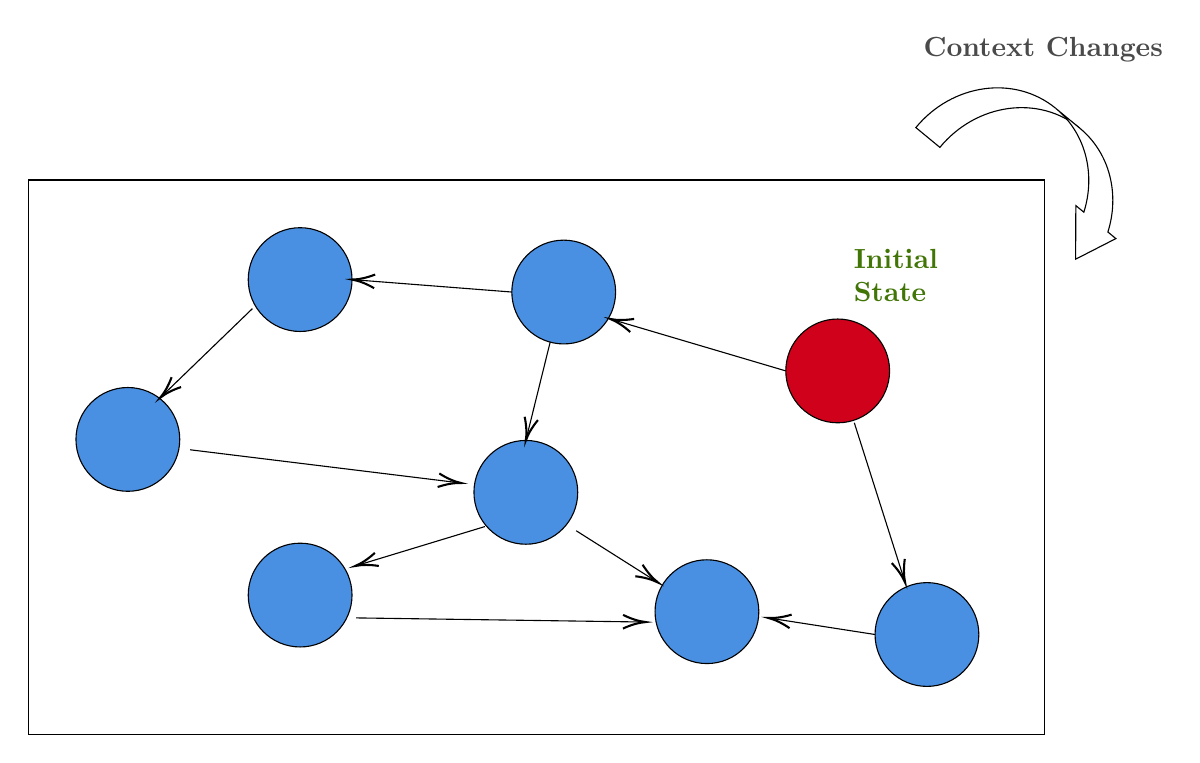
\begin{tikzpicture}[x=0.75pt,y=0.75pt,yscale=-1,xscale=1]
%uncomment if require: \path (0,410); %set diagram left start at 0, and has height of 410

%Shape: Circle [id:dp968464533790854] 
\draw  [fill={rgb, 255:red, 74; green, 144; blue, 226 }  ,fill opacity=1 ] (86,252) .. controls (86,238.19) and (97.19,227) .. (111,227) .. controls (124.81,227) and (136,238.19) .. (136,252) .. controls (136,265.81) and (124.81,277) .. (111,277) .. controls (97.19,277) and (86,265.81) .. (86,252) -- cycle ;
%Shape: Circle [id:dp21079560716947265] 
\draw  [fill={rgb, 255:red, 74; green, 144; blue, 226 }  ,fill opacity=1 ] (169,175) .. controls (169,161.19) and (180.19,150) .. (194,150) .. controls (207.81,150) and (219,161.19) .. (219,175) .. controls (219,188.81) and (207.81,200) .. (194,200) .. controls (180.19,200) and (169,188.81) .. (169,175) -- cycle ;
%Shape: Circle [id:dp5696445214135205] 
\draw  [fill={rgb, 255:red, 74; green, 144; blue, 226 }  ,fill opacity=1 ] (277.75,277.5) .. controls (277.75,263.69) and (288.94,252.5) .. (302.75,252.5) .. controls (316.56,252.5) and (327.75,263.69) .. (327.75,277.5) .. controls (327.75,291.31) and (316.56,302.5) .. (302.75,302.5) .. controls (288.94,302.5) and (277.75,291.31) .. (277.75,277.5) -- cycle ;
%Shape: Circle [id:dp5455636995208739] 
\draw  [fill={rgb, 255:red, 74; green, 144; blue, 226 }  ,fill opacity=1 ] (296,181) .. controls (296,167.19) and (307.19,156) .. (321,156) .. controls (334.81,156) and (346,167.19) .. (346,181) .. controls (346,194.81) and (334.81,206) .. (321,206) .. controls (307.19,206) and (296,194.81) .. (296,181) -- cycle ;
%Shape: Circle [id:dp8552239767397927] 
\draw  [fill={rgb, 255:red, 74; green, 144; blue, 226 }  ,fill opacity=1 ] (365,335) .. controls (365,321.19) and (376.19,310) .. (390,310) .. controls (403.81,310) and (415,321.19) .. (415,335) .. controls (415,348.81) and (403.81,360) .. (390,360) .. controls (376.19,360) and (365,348.81) .. (365,335) -- cycle ;
%Shape: Circle [id:dp49191057165067265] 
\draw  [fill={rgb, 255:red, 74; green, 144; blue, 226 }  ,fill opacity=1 ] (169,327) .. controls (169,313.19) and (180.19,302) .. (194,302) .. controls (207.81,302) and (219,313.19) .. (219,327) .. controls (219,340.81) and (207.81,352) .. (194,352) .. controls (180.19,352) and (169,340.81) .. (169,327) -- cycle ;
%Shape: Circle [id:dp20608492254875044] 
\draw  [fill={rgb, 255:red, 208; green, 2; blue, 27 }  ,fill opacity=1 ] (428,219) .. controls (428,205.19) and (439.19,194) .. (453,194) .. controls (466.81,194) and (478,205.19) .. (478,219) .. controls (478,232.81) and (466.81,244) .. (453,244) .. controls (439.19,244) and (428,232.81) .. (428,219) -- cycle ;
%Shape: Circle [id:dp40553529103941544] 
\draw  [fill={rgb, 255:red, 74; green, 144; blue, 226 }  ,fill opacity=1 ] (471,346) .. controls (471,332.19) and (482.19,321) .. (496,321) .. controls (509.81,321) and (521,332.19) .. (521,346) .. controls (521,359.81) and (509.81,371) .. (496,371) .. controls (482.19,371) and (471,359.81) .. (471,346) -- cycle ;
%Shape: Rectangle [id:dp38120662974853003] 
\draw   (63,127) -- (552.5,127) -- (552.5,394) -- (63,394) -- cycle ;
%Curve Right Arrow [id:dp7533641321758576] 
\draw  [fill={rgb, 255:red, 255; green, 255; blue, 255 }  ,fill opacity=1 ] (569.61,102.03) .. controls (549.95,85.84) and (519.78,89.99) .. (502.23,111.3) -- (490.65,101.76) .. controls (508.21,80.45) and (538.38,76.3) .. (558.04,92.49) ;\draw  [fill={rgb, 255:red, 255; green, 255; blue, 255 }  ,fill opacity=1 ] (558.04,92.49) .. controls (572.63,104.52) and (577.33,124.37) .. (571.59,142.53) -- (567.73,139.35) -- (567.63,165.17) -- (587.03,155.25) -- (583.17,152.07) .. controls (588.91,133.91) and (584.21,114.05) .. (569.61,102.03)(558.04,92.49) -- (569.61,102.03) ;
%Straight Lines [id:da45116496903786085] 
\draw    (428,219) -- (345.42,194.57) ;
\draw [shift={(343.5,194)}, rotate = 376.48] [color={rgb, 255:red, 0; green, 0; blue, 0 }  ][line width=0.75]    (10.93,-3.29) .. controls (6.95,-1.4) and (3.31,-0.3) .. (0,0) .. controls (3.31,0.3) and (6.95,1.4) .. (10.93,3.29)   ;

%Straight Lines [id:da8381673912380784] 
\draw    (461,244) -- (484.89,319.09) ;
\draw [shift={(485.5,321)}, rotate = 252.35] [color={rgb, 255:red, 0; green, 0; blue, 0 }  ][line width=0.75]    (10.93,-3.29) .. controls (6.95,-1.4) and (3.31,-0.3) .. (0,0) .. controls (3.31,0.3) and (6.95,1.4) .. (10.93,3.29)   ;

%Straight Lines [id:da23750816212213466] 
\draw    (314.5,205) -- (303.23,250.56) ;
\draw [shift={(302.75,252.5)}, rotate = 283.89] [color={rgb, 255:red, 0; green, 0; blue, 0 }  ][line width=0.75]    (10.93,-3.29) .. controls (6.95,-1.4) and (3.31,-0.3) .. (0,0) .. controls (3.31,0.3) and (6.95,1.4) .. (10.93,3.29)   ;

%Straight Lines [id:da6294824227594729] 
\draw    (296,181) -- (220.99,175.16) ;
\draw [shift={(219,175)}, rotate = 364.46000000000004] [color={rgb, 255:red, 0; green, 0; blue, 0 }  ][line width=0.75]    (10.93,-3.29) .. controls (6.95,-1.4) and (3.31,-0.3) .. (0,0) .. controls (3.31,0.3) and (6.95,1.4) .. (10.93,3.29)   ;

%Straight Lines [id:da6540760497789329] 
\draw    (327,296) -- (364.81,319.93) ;
\draw [shift={(366.5,321)}, rotate = 212.32999999999998] [color={rgb, 255:red, 0; green, 0; blue, 0 }  ][line width=0.75]    (10.93,-3.29) .. controls (6.95,-1.4) and (3.31,-0.3) .. (0,0) .. controls (3.31,0.3) and (6.95,1.4) .. (10.93,3.29)   ;

%Straight Lines [id:da5361265889850119] 
\draw    (141,257) -- (269.51,272.76) ;
\draw [shift={(271.5,273)}, rotate = 186.99] [color={rgb, 255:red, 0; green, 0; blue, 0 }  ][line width=0.75]    (10.93,-3.29) .. controls (6.95,-1.4) and (3.31,-0.3) .. (0,0) .. controls (3.31,0.3) and (6.95,1.4) .. (10.93,3.29)   ;

%Straight Lines [id:da32929255404267344] 
\draw    (283,294) -- (222.41,312.42) ;
\draw [shift={(220.5,313)}, rotate = 343.09000000000003] [color={rgb, 255:red, 0; green, 0; blue, 0 }  ][line width=0.75]    (10.93,-3.29) .. controls (6.95,-1.4) and (3.31,-0.3) .. (0,0) .. controls (3.31,0.3) and (6.95,1.4) .. (10.93,3.29)   ;

%Straight Lines [id:da6958525485352803] 
\draw    (171,189) -- (127.94,230.61) ;
\draw [shift={(126.5,232)}, rotate = 315.98] [color={rgb, 255:red, 0; green, 0; blue, 0 }  ][line width=0.75]    (10.93,-3.29) .. controls (6.95,-1.4) and (3.31,-0.3) .. (0,0) .. controls (3.31,0.3) and (6.95,1.4) .. (10.93,3.29)   ;

%Straight Lines [id:da9458308539790845] 
\draw    (221,338) -- (358.5,339.97) ;
\draw [shift={(360.5,340)}, rotate = 180.82] [color={rgb, 255:red, 0; green, 0; blue, 0 }  ][line width=0.75]    (10.93,-3.29) .. controls (6.95,-1.4) and (3.31,-0.3) .. (0,0) .. controls (3.31,0.3) and (6.95,1.4) .. (10.93,3.29)   ;

%Straight Lines [id:da834737203337281] 
\draw    (471,346) -- (421.48,338.31) ;
\draw [shift={(419.5,338)}, rotate = 368.83000000000004] [color={rgb, 255:red, 0; green, 0; blue, 0 }  ][line width=0.75]    (10.93,-3.29) .. controls (6.95,-1.4) and (3.31,-0.3) .. (0,0) .. controls (3.31,0.3) and (6.95,1.4) .. (10.93,3.29)   ;


% Text Node
\draw (552,64) node [color={rgb, 255:red, 74; green, 74; blue, 74 }  ,opacity=1 ] [align=left] {\textbf{Context Changes}};
% Text Node
\draw (481,173) node [color={rgb, 255:red, 65; green, 117; blue, 5 }  ,opacity=1 ] [align=left] {\textbf{Initial }\\\textbf{State}};


\end{tikzpicture}
}
\caption{DSPL reconfiguration with context changes}
\end{figure}

Basically, DSPL is an approach to SAS that can be incremented with a feedback loop to deal with constant environment and requirements change that were not previewed at design time \cite{SAS100-04}.



%%%%%%%%%%%%%%%%%%%%%%%%%%%%%%%%%
%%%%% SECTION %%%%%%%%%%%%%%%%%%%
%%%%%%%%%%%%%%%%%%%%%%%%%%%%%%%%%

\section {Transition System}


The TS resulted from \ref{CS01} unfolded is a set of tuples in the form:

\begin{equation}
\label{CS02}
    TS(CS_{C2})=\langle l_{C2A}, l_{TA}, l_{EX_k}, \eta, \xi \rangle |_{k=1}^n
\end{equation}

where $l_p$ is the locate $l$ for the PG $p$, $\eta \in Eval(val)$ is the value of all variables in TS and $\xi$ is the state of all channels in the system, i.e., $lenght(\xi(c)) \leq cap(c), c \in \{c_1, c_2, m_1, ..., m_n, fb\}$.

According to possible situations considered and listed in Table \ref{table:scenarios}, we can unfold the PGs above and create the related TS.

\begin{figure}[h!]
\centering
\label{TS01}
\scalebox{.8}{


\tikzset{every picture/.style={line width=0.75pt}} %set default line width to 0.75pt        

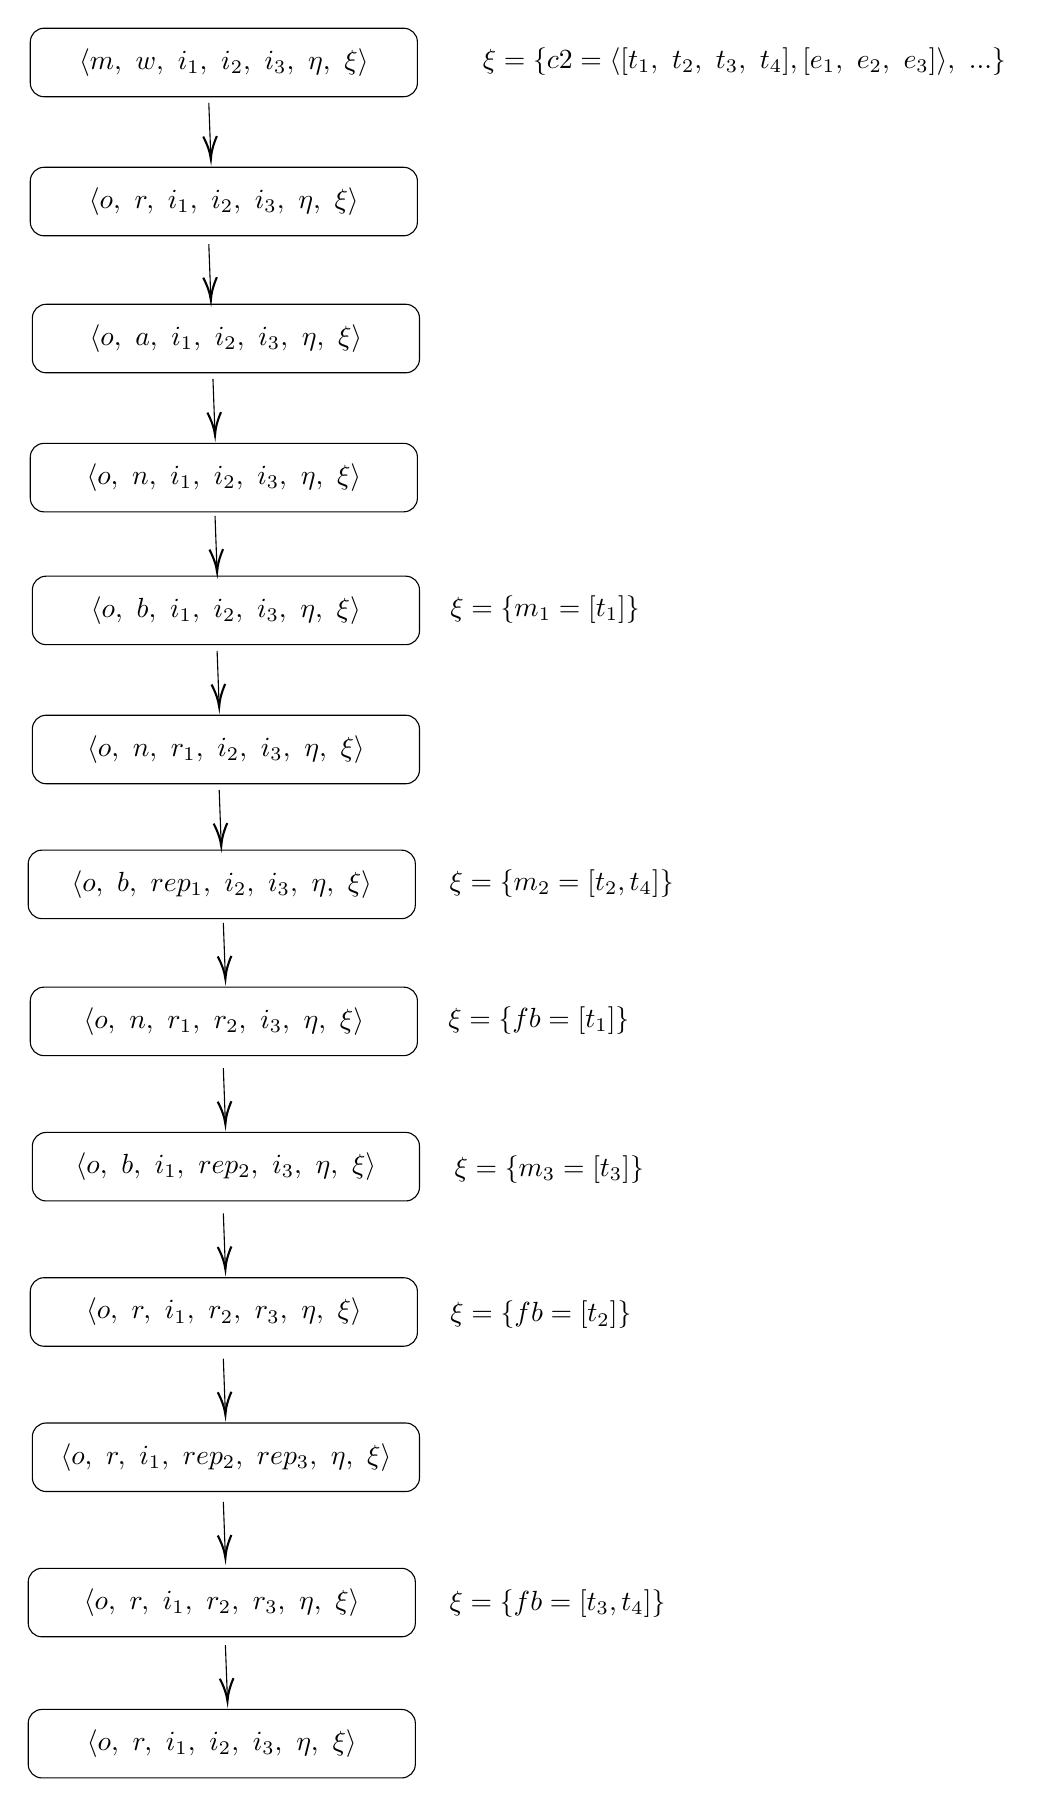
\begin{tikzpicture}[x=0.75pt,y=0.75pt,yscale=-1,xscale=1]
%uncomment if require: \path (0,865); %set diagram left start at 0, and has height of 865

%Rounded Rect [id:dp9048297129007524] 
\draw   (19,13.6) .. controls (19,9.95) and (21.95,7) .. (25.6,7) -- (198.9,7) .. controls (202.55,7) and (205.5,9.95) .. (205.5,13.6) -- (205.5,33.4) .. controls (205.5,37.05) and (202.55,40) .. (198.9,40) -- (25.6,40) .. controls (21.95,40) and (19,37.05) .. (19,33.4) -- cycle ;
%Rounded Rect [id:dp8152798292363221] 
\draw   (19,80.6) .. controls (19,76.95) and (21.95,74) .. (25.6,74) -- (198.9,74) .. controls (202.55,74) and (205.5,76.95) .. (205.5,80.6) -- (205.5,100.4) .. controls (205.5,104.05) and (202.55,107) .. (198.9,107) -- (25.6,107) .. controls (21.95,107) and (19,104.05) .. (19,100.4) -- cycle ;
%Rounded Rect [id:dp2611238064001401] 
\draw   (20,146.6) .. controls (20,142.95) and (22.95,140) .. (26.6,140) -- (199.9,140) .. controls (203.55,140) and (206.5,142.95) .. (206.5,146.6) -- (206.5,166.4) .. controls (206.5,170.05) and (203.55,173) .. (199.9,173) -- (26.6,173) .. controls (22.95,173) and (20,170.05) .. (20,166.4) -- cycle ;
%Rounded Rect [id:dp5474323622335151] 
\draw   (19,213.6) .. controls (19,209.95) and (21.95,207) .. (25.6,207) -- (198.9,207) .. controls (202.55,207) and (205.5,209.95) .. (205.5,213.6) -- (205.5,233.4) .. controls (205.5,237.05) and (202.55,240) .. (198.9,240) -- (25.6,240) .. controls (21.95,240) and (19,237.05) .. (19,233.4) -- cycle ;
%Rounded Rect [id:dp617967347556163] 
\draw   (20,277.6) .. controls (20,273.95) and (22.95,271) .. (26.6,271) -- (199.9,271) .. controls (203.55,271) and (206.5,273.95) .. (206.5,277.6) -- (206.5,297.4) .. controls (206.5,301.05) and (203.55,304) .. (199.9,304) -- (26.6,304) .. controls (22.95,304) and (20,301.05) .. (20,297.4) -- cycle ;
%Rounded Rect [id:dp6526355611328125] 
\draw   (20,344.6) .. controls (20,340.95) and (22.95,338) .. (26.6,338) -- (199.9,338) .. controls (203.55,338) and (206.5,340.95) .. (206.5,344.6) -- (206.5,364.4) .. controls (206.5,368.05) and (203.55,371) .. (199.9,371) -- (26.6,371) .. controls (22.95,371) and (20,368.05) .. (20,364.4) -- cycle ;
%Rounded Rect [id:dp6698610095556133] 
\draw   (18,409.6) .. controls (18,405.95) and (20.95,403) .. (24.6,403) -- (197.9,403) .. controls (201.55,403) and (204.5,405.95) .. (204.5,409.6) -- (204.5,429.4) .. controls (204.5,433.05) and (201.55,436) .. (197.9,436) -- (24.6,436) .. controls (20.95,436) and (18,433.05) .. (18,429.4) -- cycle ;
%Rounded Rect [id:dp9742586895494759] 
\draw   (19,475.6) .. controls (19,471.95) and (21.95,469) .. (25.6,469) -- (198.9,469) .. controls (202.55,469) and (205.5,471.95) .. (205.5,475.6) -- (205.5,495.4) .. controls (205.5,499.05) and (202.55,502) .. (198.9,502) -- (25.6,502) .. controls (21.95,502) and (19,499.05) .. (19,495.4) -- cycle ;
%Rounded Rect [id:dp34832491140564725] 
\draw   (20,545.6) .. controls (20,541.95) and (22.95,539) .. (26.6,539) -- (199.9,539) .. controls (203.55,539) and (206.5,541.95) .. (206.5,545.6) -- (206.5,565.4) .. controls (206.5,569.05) and (203.55,572) .. (199.9,572) -- (26.6,572) .. controls (22.95,572) and (20,569.05) .. (20,565.4) -- cycle ;
%Rounded Rect [id:dp07632153248409779] 
\draw   (19,615.6) .. controls (19,611.95) and (21.95,609) .. (25.6,609) -- (198.9,609) .. controls (202.55,609) and (205.5,611.95) .. (205.5,615.6) -- (205.5,635.4) .. controls (205.5,639.05) and (202.55,642) .. (198.9,642) -- (25.6,642) .. controls (21.95,642) and (19,639.05) .. (19,635.4) -- cycle ;
%Rounded Rect [id:dp38638906596830014] 
\draw   (20,685.6) .. controls (20,681.95) and (22.95,679) .. (26.6,679) -- (199.9,679) .. controls (203.55,679) and (206.5,681.95) .. (206.5,685.6) -- (206.5,705.4) .. controls (206.5,709.05) and (203.55,712) .. (199.9,712) -- (26.6,712) .. controls (22.95,712) and (20,709.05) .. (20,705.4) -- cycle ;
%Rounded Rect [id:dp2961818663412775] 
\draw   (18,755.6) .. controls (18,751.95) and (20.95,749) .. (24.6,749) -- (197.9,749) .. controls (201.55,749) and (204.5,751.95) .. (204.5,755.6) -- (204.5,775.4) .. controls (204.5,779.05) and (201.55,782) .. (197.9,782) -- (24.6,782) .. controls (20.95,782) and (18,779.05) .. (18,775.4) -- cycle ;
%Rounded Rect [id:dp1419509373702863] 
\draw   (18,823.6) .. controls (18,819.95) and (20.95,817) .. (24.6,817) -- (197.9,817) .. controls (201.55,817) and (204.5,819.95) .. (204.5,823.6) -- (204.5,843.4) .. controls (204.5,847.05) and (201.55,850) .. (197.9,850) -- (24.6,850) .. controls (20.95,850) and (18,847.05) .. (18,843.4) -- cycle ;
%Straight Lines [id:da25623652531692265] 
\draw    (105,43) -- (105.93,68) ;
\draw [shift={(106,70)}, rotate = 267.88] [color={rgb, 255:red, 0; green, 0; blue, 0 }  ][line width=0.75]    (10.93,-3.29) .. controls (6.95,-1.4) and (3.31,-0.3) .. (0,0) .. controls (3.31,0.3) and (6.95,1.4) .. (10.93,3.29)   ;
%Straight Lines [id:da9454848916406987] 
\draw    (105,111) -- (105.93,136) ;
\draw [shift={(106,138)}, rotate = 267.88] [color={rgb, 255:red, 0; green, 0; blue, 0 }  ][line width=0.75]    (10.93,-3.29) .. controls (6.95,-1.4) and (3.31,-0.3) .. (0,0) .. controls (3.31,0.3) and (6.95,1.4) .. (10.93,3.29)   ;
%Straight Lines [id:da9308850791504091] 
\draw    (107,176) -- (107.93,201) ;
\draw [shift={(108,203)}, rotate = 267.88] [color={rgb, 255:red, 0; green, 0; blue, 0 }  ][line width=0.75]    (10.93,-3.29) .. controls (6.95,-1.4) and (3.31,-0.3) .. (0,0) .. controls (3.31,0.3) and (6.95,1.4) .. (10.93,3.29)   ;
%Straight Lines [id:da6987828125639035] 
\draw    (108,242) -- (108.93,267) ;
\draw [shift={(109,269)}, rotate = 267.88] [color={rgb, 255:red, 0; green, 0; blue, 0 }  ][line width=0.75]    (10.93,-3.29) .. controls (6.95,-1.4) and (3.31,-0.3) .. (0,0) .. controls (3.31,0.3) and (6.95,1.4) .. (10.93,3.29)   ;
%Straight Lines [id:da38465000460546606] 
\draw    (109,307) -- (109.93,332) ;
\draw [shift={(110,334)}, rotate = 267.88] [color={rgb, 255:red, 0; green, 0; blue, 0 }  ][line width=0.75]    (10.93,-3.29) .. controls (6.95,-1.4) and (3.31,-0.3) .. (0,0) .. controls (3.31,0.3) and (6.95,1.4) .. (10.93,3.29)   ;
%Straight Lines [id:da7402304756808019] 
\draw    (110,374) -- (110.93,399) ;
\draw [shift={(111,401)}, rotate = 267.88] [color={rgb, 255:red, 0; green, 0; blue, 0 }  ][line width=0.75]    (10.93,-3.29) .. controls (6.95,-1.4) and (3.31,-0.3) .. (0,0) .. controls (3.31,0.3) and (6.95,1.4) .. (10.93,3.29)   ;
%Straight Lines [id:da32843301316145035] 
\draw    (112,438) -- (112.93,463) ;
\draw [shift={(113,465)}, rotate = 267.88] [color={rgb, 255:red, 0; green, 0; blue, 0 }  ][line width=0.75]    (10.93,-3.29) .. controls (6.95,-1.4) and (3.31,-0.3) .. (0,0) .. controls (3.31,0.3) and (6.95,1.4) .. (10.93,3.29)   ;
%Straight Lines [id:da33931279270538006] 
\draw    (112,508) -- (112.93,533) ;
\draw [shift={(113,535)}, rotate = 267.88] [color={rgb, 255:red, 0; green, 0; blue, 0 }  ][line width=0.75]    (10.93,-3.29) .. controls (6.95,-1.4) and (3.31,-0.3) .. (0,0) .. controls (3.31,0.3) and (6.95,1.4) .. (10.93,3.29)   ;
%Straight Lines [id:da4793309632596934] 
\draw    (112,578) -- (112.93,603) ;
\draw [shift={(113,605)}, rotate = 267.88] [color={rgb, 255:red, 0; green, 0; blue, 0 }  ][line width=0.75]    (10.93,-3.29) .. controls (6.95,-1.4) and (3.31,-0.3) .. (0,0) .. controls (3.31,0.3) and (6.95,1.4) .. (10.93,3.29)   ;
%Straight Lines [id:da7517013161282193] 
\draw    (112,648) -- (112.93,673) ;
\draw [shift={(113,675)}, rotate = 267.88] [color={rgb, 255:red, 0; green, 0; blue, 0 }  ][line width=0.75]    (10.93,-3.29) .. controls (6.95,-1.4) and (3.31,-0.3) .. (0,0) .. controls (3.31,0.3) and (6.95,1.4) .. (10.93,3.29)   ;
%Straight Lines [id:da06264248753342316] 
\draw    (112,717) -- (112.93,742) ;
\draw [shift={(113,744)}, rotate = 267.88] [color={rgb, 255:red, 0; green, 0; blue, 0 }  ][line width=0.75]    (10.93,-3.29) .. controls (6.95,-1.4) and (3.31,-0.3) .. (0,0) .. controls (3.31,0.3) and (6.95,1.4) .. (10.93,3.29)   ;
%Straight Lines [id:da8026456818678067] 
\draw    (113,786) -- (113.93,811) ;
\draw [shift={(114,813)}, rotate = 267.88] [color={rgb, 255:red, 0; green, 0; blue, 0 }  ][line width=0.75]    (10.93,-3.29) .. controls (6.95,-1.4) and (3.31,-0.3) .. (0,0) .. controls (3.31,0.3) and (6.95,1.4) .. (10.93,3.29)   ;

% Text Node
\draw (112.25,23.5) node    {$\langle m,\ w,\ i_{1} ,\ i_{2} ,\ i_{3} ,\ \eta ,\ \xi \rangle $};
% Text Node
\draw (112.25,90.5) node    {$\langle o,\ r,\ i_{1} ,\ i_{2} ,\ i_{3} ,\ \eta ,\ \xi \rangle $};
% Text Node
\draw (363,23) node    {$\xi =\{c2=\langle [ t_{1} ,\ t_{2} ,\ t_{3} ,\ t_{4}] ,[ e_{1} ,\ e_{2} ,\ e_{3}] \rangle ,\ ...\}$};
% Text Node
\draw (113.25,156.5) node    {$\langle o,\ a,\ i_{1} ,\ i_{2} ,\ i_{3} ,\ \eta ,\ \xi \rangle $};
% Text Node
\draw (112.25,223.5) node    {$\langle o,\ n,\ i_{1} ,\ i_{2} ,\ i_{3} ,\ \eta ,\ \xi \rangle $};
% Text Node
\draw (113.25,287.5) node    {$\langle o,\ b,\ i_{1} ,\ i_{2} ,\ i_{3} ,\ \eta ,\ \xi \rangle $};
% Text Node
\draw (267,287) node    {$\xi =\{m_{1} =[ t_{1}]\}$};
% Text Node
\draw (113.25,354.5) node    {$\langle o,\ n,\ r_{1} ,\ i_{2} ,\ i_{3} ,\ \eta ,\ \xi \rangle $};
% Text Node
\draw (111.25,419.5) node    {$\langle o,\ b,\ rep_{1} ,\ i_{2} ,\ i_{3} ,\ \eta ,\ \xi \rangle $};
% Text Node
\draw (275,419) node    {$\xi =\{m_{2} =[ t_{2} ,t_{4}]\}$};
% Text Node
\draw (112.25,485.5) node    {$\langle o,\ n,\ r_{1} ,\ r_{2} ,\ i_{3} ,\ \eta ,\ \xi \rangle $};
% Text Node
\draw (113.25,555.5) node    {$\langle o,\ b,\ i_{1} ,\ rep_{2} ,\ i_{3} ,\ \eta ,\ \xi \rangle $};
% Text Node
\draw (269,557) node    {$\xi =\{m_{3} =[ t_{3}]\}$};
% Text Node
\draw (112.25,625.5) node    {$\langle o,\ r,\ i_{1} ,\ r_{2} ,\ r_{3} ,\ \eta ,\ \xi \rangle $};
% Text Node
\draw (113.25,695.5) node    {$\langle o,\ r,\ i_{1} ,\ rep_{2} ,\ rep_{3} ,\ \eta ,\ \xi \rangle $};
% Text Node
\draw (111.25,765.5) node    {$\langle o,\ r,\ i_{1} ,\ r_{2} ,\ r_{3} ,\ \eta ,\ \xi \rangle $};
% Text Node
\draw (111.25,833.5) node    {$\langle o,\ r,\ i_{1} ,\ i_{2} ,\ i_{3} ,\ \eta ,\ \xi \rangle $};
% Text Node
\draw (265,627) node    {$\xi =\{fb=[ t_{2}]\}$};
% Text Node
\draw (264,485) node    {$\xi =\{fb=[ t_{1}]\}$};
% Text Node
\draw (273,766) node    {$\xi =\{fb=[ t_{3} ,t_{4}]\}$};


\end{tikzpicture}}
\caption{TS for the Normal execution}
\end{figure}


%%%%%%%%%%%%%%%%%%%%%%%%%%%%%%%%%
%%%%% SECTION %%%%%%%%%%%%%%%%%%%
%%%%%%%%%%%%%%%%%%%%%%%%%%%%%%%%%

\section {Program Graph}

The model used to represent the behavior of a system is called Transition System (TS). It is a representation of all possible states that a system can reach during the execution. A TS can be written as tuple show in Equation \ref{TS01} .

\begin{center}
\begin{equation}
        TS_{k} = (S, Act, I, \longrightarrow, AP ,L)
        \label{TS01}
    \end{equation}
\end{center}

where $S$ is the set of states that the system can adopt. The $Act$ represents a set of actions executed where the system changes its state. The $I \subseteq S$ is the initial states set. The transition relation $(\longrightarrow \subseteq S \times Act \times S)$ links valid states representing these changes. The set of atomic propositions $AP$ manipulated by the constraints formulas. And the labels set $L$ is labeling function that assigns identifiers to the states, and is defined as $L:S \longrightarrow 2^{AP}$.

The behavior of a TS that starts in a initial state $s_0 \in I \subseteq S$ can be represented as $s_i \xrightarrow[]{\alpha} s_j$ where $s_i$ is the current state, $\alpha \in Act$ is the action that conducts to the new state $s_j$. In addition, we can have data-dependent system, where the action depends on the results of some conditional expression in the form $s_i \xrightarrow[]{g:\alpha} s_j$ where $g$ is a Boolean typed and called guard condition. The TS will be resulted from unfolded graph with all possible paths according to the boolean expression result\cite{baier}.

However, the representation using TS can be unfeasible due to the number of all possible states that a component can adopt. Thereby, we will use Program graph representation to turn able a whole view of the system and execution steps. It is an abstraction which encapsulates the conditional expression with data dependence. A Program Graph (PG) is applied over a set of typed variables and it is represented by the following tuple:

\begin{center}
    $(Loc,Act,Effect,\lhookrightarrow,Loc_0,g_0)$
\end{center}

where,

\begin{itemize}
	\item $Loc$ is a set of location  
	\item $Act$ is a set of actions
	\item Effect is a function whose type is $Act \times Eval(Var) \to Eval(Var)$
	\item $\lhookrightarrow$ is the conditional transition relation defined by $Loc \times Cond(Var) \times Act \times Loc$
	\item $Loc_0 \subseteq Loc$ is the set of initial locations
	\item $g_0 \in Cond(Var)$ is the initial condition
\end{itemize}

However, in modern computation we do not have a sequential execution of a number of PGs. Normally, we have a set of processes represented by program graphs that run in a parallel way. Based on this, the PGs must be able to run in parallel and, in some cases, to be able to synchronize with each other. We can have the PGs running synchronously, i.e., performing a handshaking, or asynchronously, i.e., via a buffer under \textit{first-in, first-out} policy.


%%%%%%%%%%%%%%%%%%%%%%%%%%%%%%%%%
%%%%% SECTION %%%%%%%%%%%%%%%%%%%
%%%%%%%%%%%%%%%%%%%%%%%%%%%%%%%%%

\section {Channel System}

A CS is a composition  of Program Graphs (PG) exploring the parallelism and communication exchanging data, i.e., sending messages, between them using communication structures called \textit{channels}\cite{baier}. This structure is called Channel System and is formed by a set of PGs extended with communication actions. The two possible operations over the channels are done with the following communication actions (from \cite{baier}):

\begin{itemize}
	\item $c!v$ is the transmission of value $v$ through the channel $c$ 
	\item $c?v$ is the receiving of value $v$ through the channel $c$
\end{itemize}

The capacity of the channel $c$, i.e., $Cap(c) \in \mathbb{N} \bigcup \{\infty\}$, defines if it is synchronous or asynchronous. A channel with the capacity equals to zero is synchronous, i.e., represents a handshaking between processes, where the transmitter process wait for the receiver reading. In that way, only one value is exchanged between two processes per time. On the other hand, an asynchronous channel has the capacity greater than zero and the process that sends the value does not need to wait the receiver process read the value written. In this case, the buffer that represents the channel works as a short memory where the process store values that will be manipulated by any other process later. This buffer works as a \textit{first-in-first-out} queue and, as long as the number of values written in the buffer is less the its capacity, it will be possible to add new values. 

With the communication resource integrated, we can define a PG over a set of variables $Var$ and a set of Channels $Chan$ as the same previous tuple $(Loc,Act,Effect,\lhookrightarrow,Loc_0,g_0)$ but with the following difference in the $\lhookrightarrow$ element:

\begin{center}
    $\lhookrightarrow \subseteq (Loc \times (Cond(Var) \times (Act \bigcup Comm) \times Loc)$
\end{center}

where \textit{(Act $\bigcup$ Comm)} extends the actions set with the communication actions described before. By combining a set with $n$ parallel PGs such that each $PG_i$ over $(Var_i, Chan)$, where $1 \leq i \leq n$, composes a Channel System (CS) over the set $(Var, Chan)$ defined as following.

\begin{center}
    $CS=[PG_1 | PG_2 | ... | PG_n]$
\end{center}

The $Var$ set of CS is defined as $\bigcup_{1 \leq i \leq n}Var_i$, i.e., the combination of all $Var_i$ sets of each $PG_i$ that composes the CS.
